\section{\ExercisePrefixEmbeddedC Touchscreen ansteuern \optional}
Eingebaut im mit dem Mikrocontroller verbundenen Bildschirm ist eine resistive 4-Wire Touchschicht.
Der Name setzt sich zusammen aus den Eigenschaften dieser Schaltung.
Resistiv steht für die Messung von Widerständen zum Erkennen von Touch-Gesten und 4-Wire, da für diese Durchführung vier Datenleitungen gebraucht werden.
Ein 4-Wire resistiver Touchscreen ist wie in \Cref{fig:rsTouch} aufgebaut.
Diese besteht aus einer Glass- oder Acryl-Schicht, einer äußeren resistiven Schicht die mit ITO (indium-tin-oxide) beschichtet ist, isolierender Punkten, der inneren resistiven Schicht aus ITO und einem Polyester-Film. Wie in Abbildung \ref{fig:fourRSTouch} dargestellt sind die beiden resistiven Schichten jeweils an 2 Polen angeschlossen. Die Schichten sind in Bezug auf ihre Pole um 90 Grad zueinander gedreht. Dies ist wichtig, um später die X- und Y-Koordinaten des Touch-Points zu lesen. Sobald ein Objekt, welches nicht leitfähig sein muss, die oberste Glaß- oder Acryl-Schicht berührt und genügend Druck ausübt, wird sich die oberste ITO-Schicht mit der unteren verbinden. Die X- und Y-Koordinate wird bestimmt, indem die Spannungen an den Polen gemessen werden. Zur Messung des X-Wertes werden X+ und X- über Gleichspannung geschaltet. Das heißt X+ ist beispielsweise auf Vcc und X- ist mit GND verbunden. Durch die Verbindung der beiden ITO-Schichten entsteht ein Stromfluss durch beide Schichten und es kommt zu einem Spannungsteiler in der X-Schicht. Die Spannungen zwischen X+ und der Druckposition und der Druckposition und X- lassen sich durch das Ausmessen von Y- und Y+ auslesen. Diese Information wird an einen Controller weitergegeben, der die gemessene Spannung in Relation zur Aufl{\"o}sung des Displays setzt. Die Y-Koordinate wird gemessen, indem Y+ und Y- an eine Gleichspannung gelegt und die Spannungen an X+ und X- ausgelesen werden. Die Library des FM4 enthält die Funktionen readTouchX(), readTouchY() und readTouchZ() die X,Y- und Z-Werte eines Berührungspunktes auf dem Touchscreen auslesen können. Ist der Z-Wert größer als ein bestimmter Threshold, kann von einer Berührung des Touchscreens ausgegangen werden. 
\begin{figure}[htbp]
    \centering
    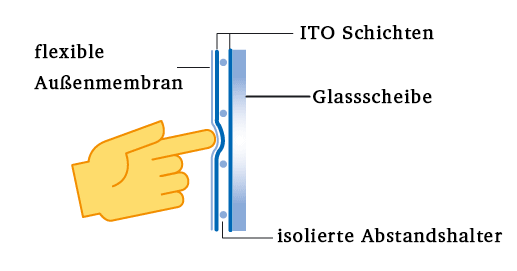
\includegraphics[width=0.35\textwidth]{./05_c/figures/4WireRSTouch.png}
    \caption{Aufbau eines resistiven Touchscreens}
    \label{fig:rsTouch}
\end{figure}
\begin{figure}[htbp]
	\centering
	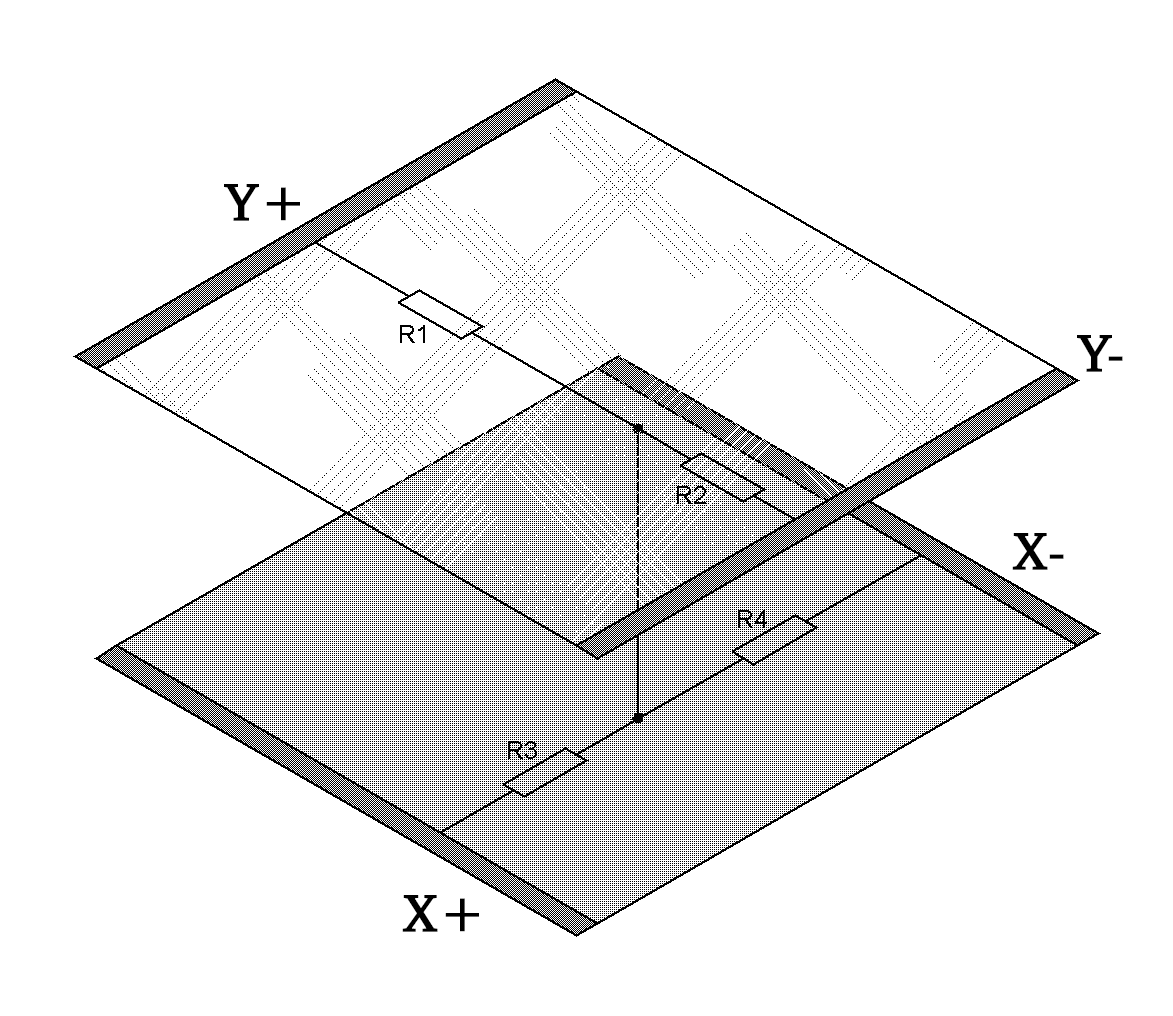
\includegraphics[width=0.3\textwidth]{./05_c/figures/ResistiveTS.png}
	\caption{Aufbau eines 4-Wire resistiven Touchscreens }
	\label{fig:fourRSTouch}
\end{figure} 

\subsection{Werte des Touchscreens debuggen}
Zunächst soll die Funktion debugTouch() implementiert werden, die kontinuierlich die X-,Y- und Z-Werte des Touchscreens auf dem Bildschirm, ähnlich zum Debugging der Joysticks, ausgibt.

\subsection{Zeichnen auf dem Touchscreen}
In diesem Abschnitt soll eine Mal-Anwendung für den Touchscreen entwickelt werden. Mit dieser soll es möglich sein verschiedene Farben auszuwählen und mit diesem per Touchgesten auf dem Bildschirm zu zeichnen. Hierfür soll die Funktion paintTouch() vervollständigt werden. Bereits implementiert sind die Farbpaletten und der Lösch-Button auf der unteren Seite des Bildschirms. Die Funktion printTouch() muss noch um eine Touch-Logik ergänzt werden, die Berührungspunkte auf dem Bildschirm erkennt und diese korrekt interpretiert. Hierbei gibt es folgende Szenarien: 
(1.) Die Farbpalette wird berührt und somit verändert sich die aktuelle Malfarbe.
(2.) Bild erneuern wurde gedrückt und der Malbereich wird zurückgesetzt.
(3.) Wird der freie Zeichen-Bereich berührt, so soll an dieser Stelle in der ausgewählten Farbe ein ausgefüllter Kreis mit dem Radius PENRADIUS gezeichnet werden.
\begin{figure}[htbp]
	\centering
	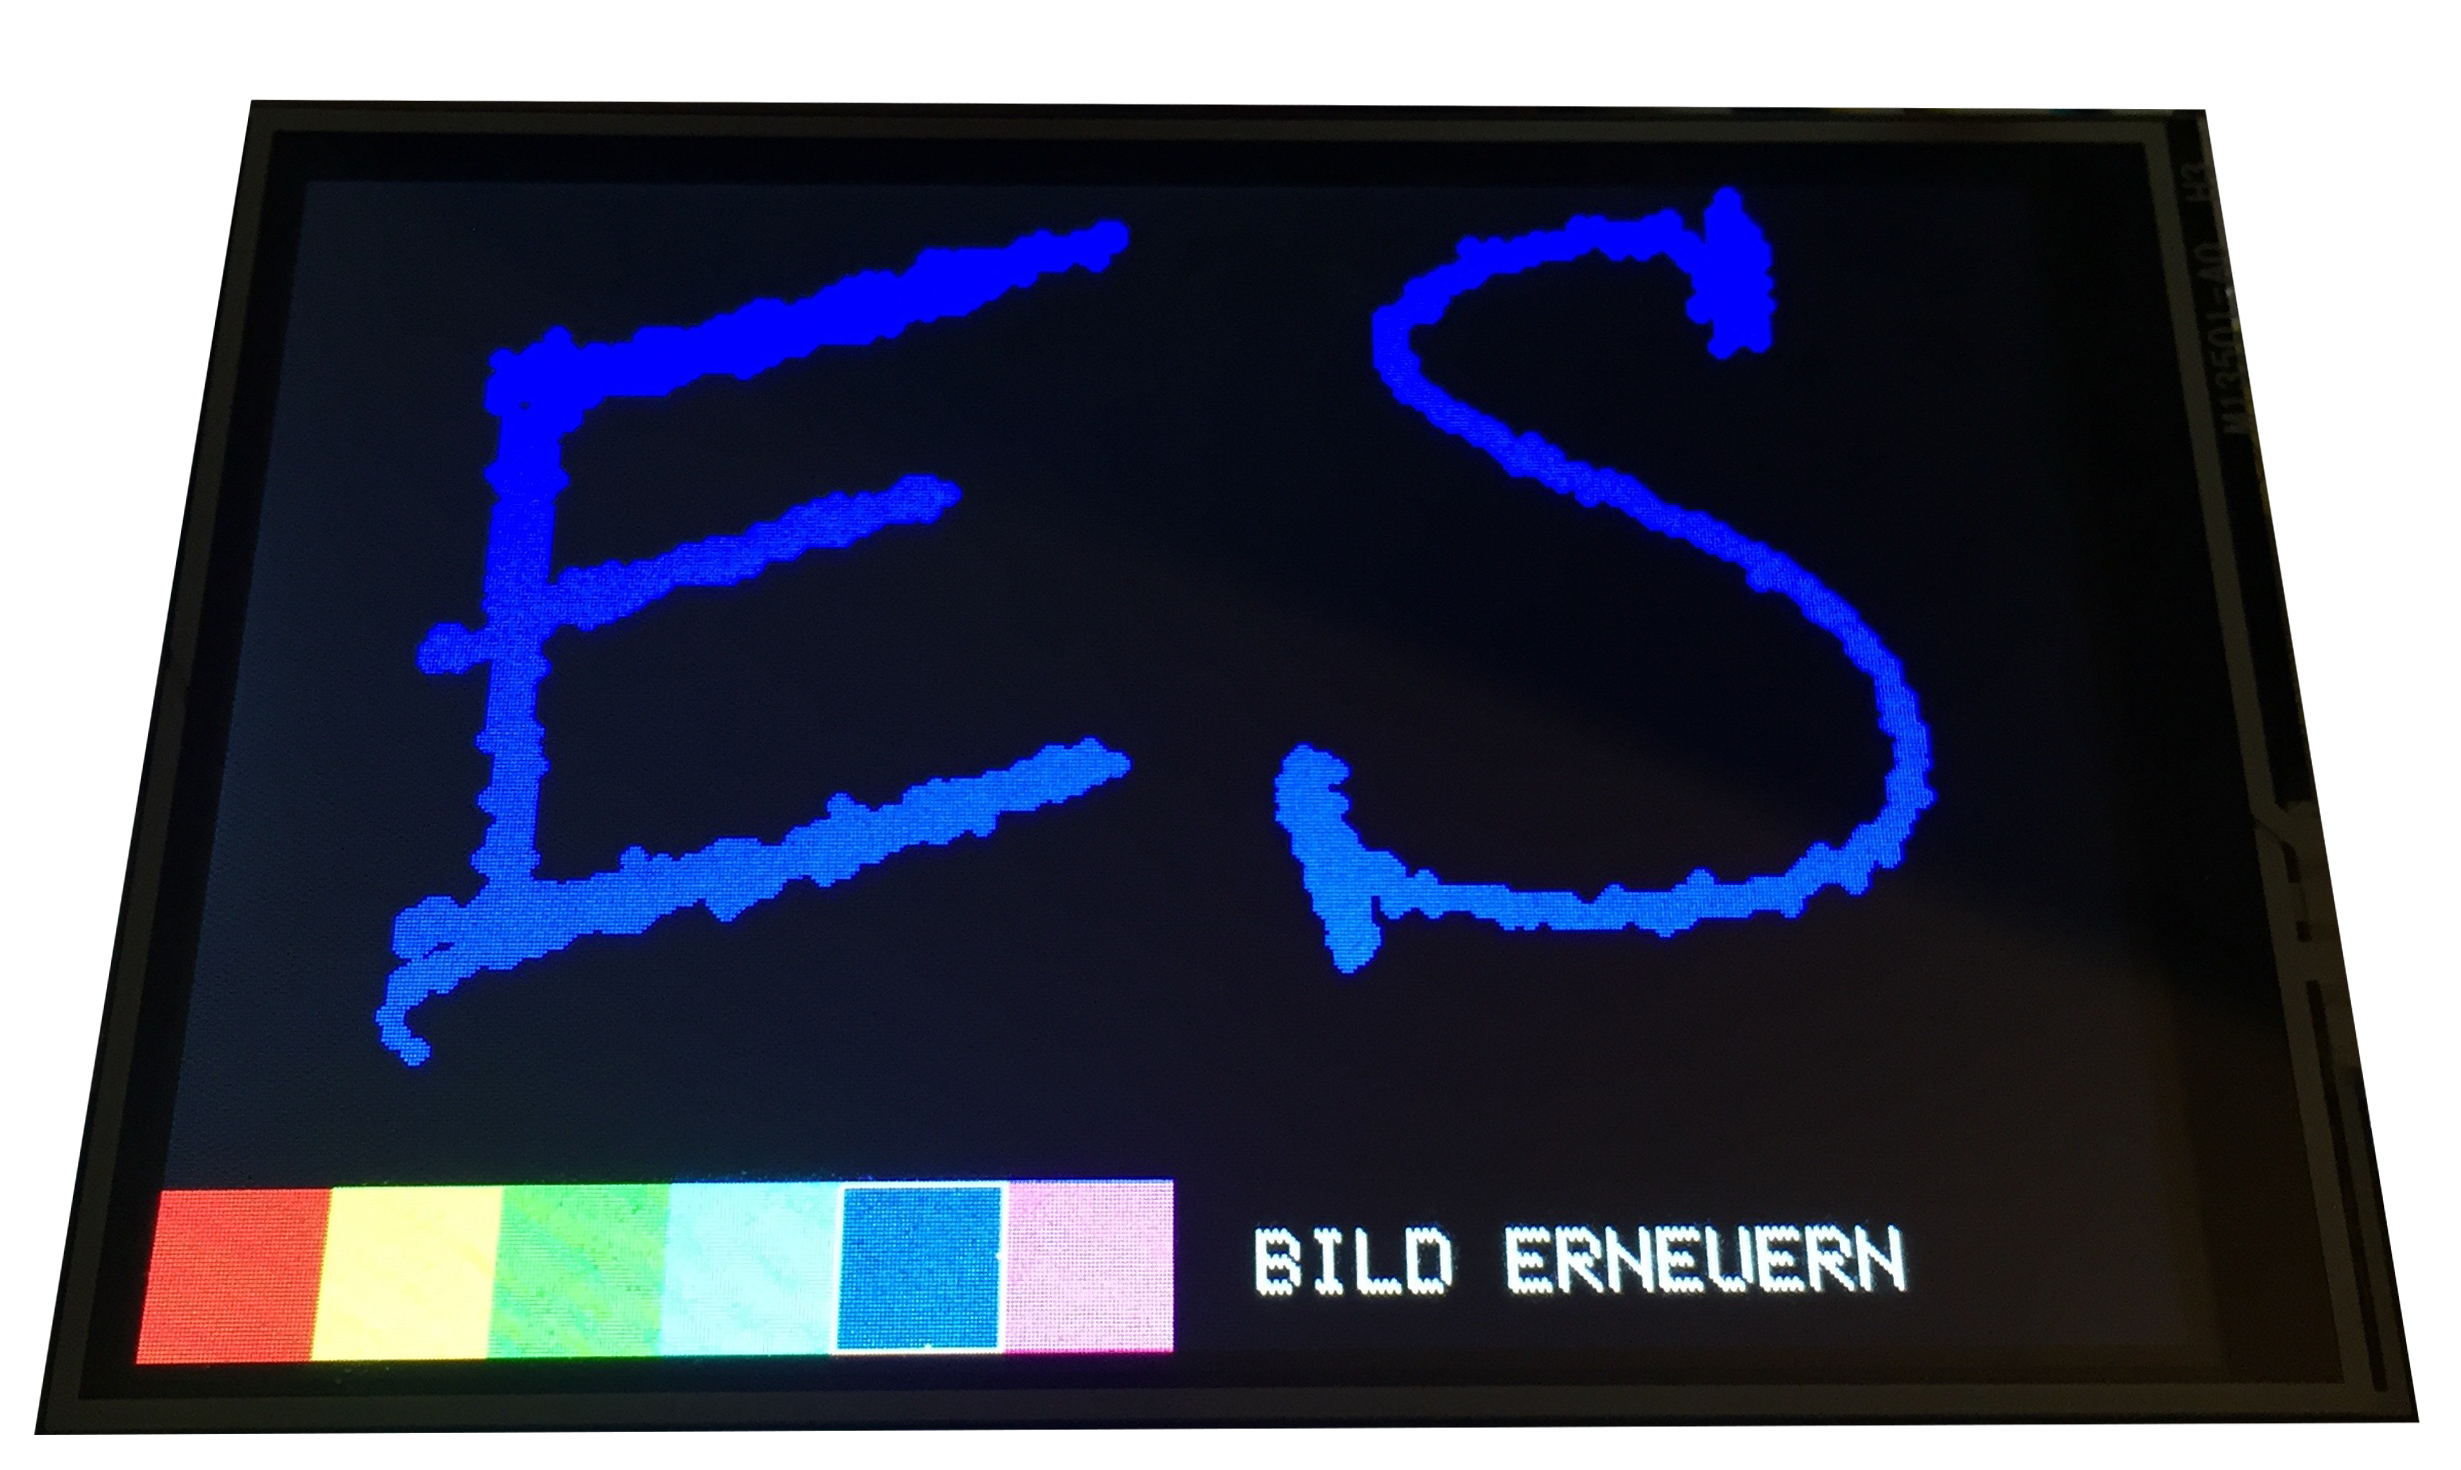
\includegraphics[width=0.3\textwidth]{./05_c/figures/Paint-Szenario.png}
	\caption{Paint-Anwendung auf dem Touchscreen}
	\label{img:paintTouch}
\end{figure} 